\subsection{Classi e Oggetti}

\begin{definition}[Oggetto]
    Un \textbf{\textcolor{cyan}{oggetto}} è un entità caratterizzata da un'\emph{\textcolor{cyan}{identità}},
    uno \emph{\textcolor{cyan}{stato}}, ovvero i valori degli \emph{attributi} dell'oggetto, e da un \emph{\textcolor{cyan}{comportamento}},
    quindi le operazioni che lo definiscono.
\end{definition}

\begin{definition}[Classe]
    Una \textbf{\textcolor{cyan}{classe}} è un insieme di \emph{oggetti} con caratteristiche simili,
    quindi che hanno lo stesso tipo.

    Una classe permette di catturare gli elementi del dominio del sistema.
\end{definition}

\subsubsection{Diagramma delle Classi}

Descrive le \textcolor{cyan}{proprietà} e le \textcolor{cyan}{operazioni} di un classe, il \textcolor{cyan}{tipo degli oggetti}, e le \textcolor{cyan}{relazioni \emph{statiche}} fra essi.

\begin{wrapfigure}{l}{0.\textwidth}
    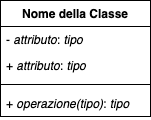
\includegraphics[scale=0.7]{img/diagrammaclassi.png}
\end{wrapfigure}

Una classe viene rappresentata in questo modo, con il nome sempre in maiuscolo, la sezione che riguarda gli attributi
e quella che riguarda le operazioni. Il simbolo \textbf{\textcolor{MidnightBlue}{$+$}} indica un attributo/operazione privata, mentre il \textbf{\textcolor{MidnightBlue}{$-$}} ne indica uno
pubblico. Esistono anche altri due simboli per la \emph{\textcolor{cyan}{visibilità}}: il \textbf{\textcolor{MidnightBlue}{$\#$}}, che indica
che l'attributo o l'operazione è accessibile anche alle classi discendenti nella \textcolor{cyan}{gerarchia}, mentre la
\textbf{\textcolor{MidnightBlue}{$\sim$}} che indica l'accessibilità solo alle classi nello stesso \emph{package}.
Inoltre, per specificare che un attributo o un'operazione sono \emph{\textcolor{cyan}{statici}}, si sottolineano.

Nonostante ciò, quando si usa il diagramma delle classi per descrivere il dominio, sia le operazioni che la visibilità
e i dettagli implementativi degli attributi si omettono.

\paragraph{Attributi} La sintassi degli attributi è la seguente:
\begin{center}
    \verb|Visibilità Nome: Tipo[Molteplicità] = ValoreDefault {Proprietà}| 
\end{center}
La \textcolor{cyan}{\emph{molteplicità}} indica gli array di valori, quando è uguale a $1$ può essere omessa.
Invece, le \textcolor{cyan}{\emph{proprietà}} possono essere sui valori dell'attributo, oppure nel caso la molteplicità è maggiore di $1$ si può
usare \verb|{ordered}| per indicare che nell'array l'ordine degli elementi conta, e \verb|{unique}| per dire che gli elementi
dell'array non devono avere ripetizioni.

\paragraph{Operazioni} La sintassi delle operazioni è la seguente:
\begin{center}
    \verb|Visibilità Nome: (ListaParametri) : TipoRitorno| 
\end{center}
Con \verb|ListaParametri| definita dalla seguente grammatica:
\[
    ListaParametri::=\;\varnothing\;|\;DichiarazioneParametro,\;ListaParametri
\]
\[
    DichiarazioneParametro::=\;Nome:\;Tipo\;=\;ValoreDefault
\]

\paragraph{Enumerazioni} Sono usate per specificare una lista prefissata di valori che un \emph{\textcolor{cyan}{attributo}} può assumere.
In UML sono etichettate con lo stereotipo \verb|<<enumeration>>|.
\begin{figure}[h]
    \centering
    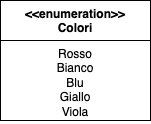
\includegraphics[scale=0.7]{img/enumeration.png}
    \caption{\begin{tabular}{c}Esempio di enumerazione con l'attributo \emph{colore}.\end{tabular}}
\end{figure}

\subsubsection{Relazioni}

\begin{definition}[Relazione]
    Una \textbf{\textcolor{cyan}{relazione}} rappresenta un legame tra due o più oggetti.

    In UML viene rappresentata da una linea retta con sopra scritte il \textcolor{cyan}{nome dell'associazione}, il \textcolor{cyan}{ruolo} di ogni classe, ed
    eventualmente una freccia che sta ad indicare il verso di lettura dell'associazione.

    In generale si usa specificare o solo il \emph{nome dell'associazione} o solo i \emph{ruoli}.
\end{definition}

\begin{figure}[h]
    \centering
    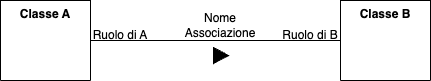
\includegraphics[scale=0.7]{img/relazione.png}
\end{figure}

\newpage
\paragraph{\textcolor{cyan}{Molteplicità}} La \emph{molteplicità} indica il numero di oggetti
coinvolti in un'associazione in un dato istante. Può essere definita in uno dei seguenti modi:
\begin{itemize}
    \item Con un numero positivo.
    \item Con \verb|*| che indica un valore indefinito.
    \item Indicando gli estremi inferiore e superiore di un intervallo (es. 2..4, 0..5, 7..*).
\end{itemize}

\begin{figure}[h]
    \centering
    \includegraphics[scale=0.7]{img/molteplicità.png}
\end{figure}

\paragraph{\textcolor{cyan}{Associazioni Riflessive}} Si riferiscono alla stessa classe e, in questo caso, è fondamentale il ruolo
dei due oggetti.

\begin{figure}[h]
    \centering
    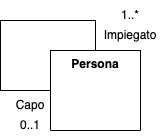
\includegraphics[scale=0.7]{img/riflessiva.png}
    \caption{Esempio di associazione riflessiva.}
\end{figure}

\newpage
\subsubsection{Aggregazione e Composizione}

L'\textbf{\textcolor{cyan}{aggregazione}} e la \textbf{\textcolor{cyan}{composizione}}
sono tipi di relazioni in cui viene specificato che un oggetto di una classe \emph{fà parte} di un oggetto
di un'altra classe. L'\emph{aggregazione} è meno forte come relazione, quindi si verifica quando le \emph{\textcolor{MidnightBlue}{classi parte}} hanno un
significato anche senza la presenza della \emph{\textcolor{MidnightBlue}{classe tutto}}. Nella \emph{composizione}, invece, la \emph{classe parte} ha un senso solo
se legata alla \emph{classe tutto}.

\begin{figure}[h]
    \centering
    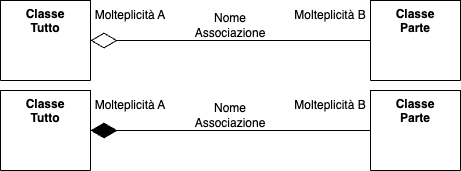
\includegraphics[scale=0.7]{img/aggrecomp.png}
    \caption{Sopra \emph{aggregazione}, sotto \emph{composizione}.}
\end{figure}

\subsubsection{Generalizzazione}
Consiste in una relazione tra una classe più generica e una più specializzata: la classe specializzata o
\emph{\textcolor{cyan}{sottoclasse}} eredita tutte le caratteristiche della \emph{\textcolor{cyan}{superclasse}}, può aggiungerne delle altre, e
può ridefinire delle \emph{operazioni}.

In questa relazione vale il \emph{Principio di Sostituzione di Liskov} \footnote{\url{https://it.wikipedia.org/wiki/Principio_di_sostituzione_di_Liskov}},
ovvero un oggetto della classe specializzata può essere usato al posto di un oggetto della superclasse.

\begin{figure}[h]
    \centering
    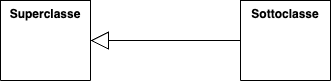
\includegraphics[scale=0.7]{img/generalizzazione.png}
\end{figure}

\newpage
\subsubsection{Classi Astratte}
Le \textbf{\textcolor{cyan}{classi astratte}} definiscono delle classi che non sono implementate completamente.

\begin{figure}[h]
    \centering
    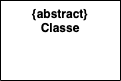
\includegraphics[scale=0.7]{img/abstract.png}
\end{figure}

\subsubsection{Interfacce}
Le \textbf{\textcolor{cyan}{interfacce}} si usano in fase di \emph{progettazione} per definire
delle classi con solo operazioni e senza attributi.

\begin{figure}[h]
    \centering
    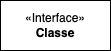
\includegraphics[scale=0.7]{img/interface.png}
\end{figure}

\paragraph{Nota Bene} Sia le \emph{interfacce} che le \emph{classi astratte} non possono essere istanziate, ma si utilizzano
nelle \emph{\textcolor{cyan}{gerarchie}} per definire la "\emph{struttura}" di classi più complete.

\subsubsection{Dipendenze}
La dipendenza è una relazione in cui le classi hanno un ruolo di
\emph{\textcolor{cyan}{cliente}} e di \emph{\textcolor{cyan}{fornitore}}. Questo avviene quando
un parametro di un'operazione della classe \emph{cliente} è un oggetto della classe \emph{fornitore}, o se un'operazione
del \emph{cliente} restituisce o crea dinamicamente un oggetto del tipo del \emph{fornitore}.

\begin{figure}[h]
    \centering
    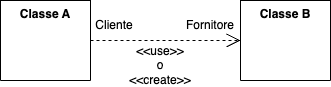
\includegraphics[scale=0.7]{img/dipendenza.png}
\end{figure}

\subsubsection{Classi Associazione}
Un'associazione può avere dei propri attributi, rappresentati con una \textbf{\textcolor{cyan}{classe associazione}}.
Per ogni coppia di classi, può esistere solo una \emph{classe associazione}.

\begin{figure}[h]
    \centering
    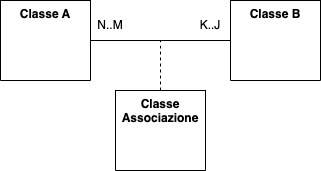
\includegraphics[scale=0.7]{img/classeass.png}
\end{figure}

\subsubsection{Classi di Analisi}
Le \textbf{\textcolor{cyan}{classi di analisi}} corrispondono ai concetti
concreti del dominio, per esempio i termini del glossario. Queste classi hanno un numero
ridotto di \emph{\textcolor{cyan}{funzionalità}} e durante la loro definizione occorre
evitare di:
\begin{itemize}
    \item Definire classi "\emph{\textcolor{cyan}{onnipotenti}}".
    \item Definire classi che in realtà sono delle \emph{\textcolor{cyan}{funzioni}}.
    \item Definire delle \emph{\textcolor{cyan}{gerarchie}} troppo profonde (più di 3 livelli).
    \item Specificare troppo i \emph{\emph{\textcolor{cyan}{tipi}}} e i \emph{\emph{\textcolor{cyan}{valori}}} degli \emph{attributi}.
\end{itemize}
Inoltre le \emph{operazioni} e gli \emph{attributi} vanno indicati solo quando sono veramente utili.

Le principali tecniche di definizione delle \emph{classi di analisi} sono:
\begin{itemize}
    \item \textcolor{cyan}{Data Driven}: durante la \emph{fase di analisi}, si identificano tutti i dati del sistema e si dividono
        in classi.
        \item \textcolor{cyan}{Responsibility Driven}: durante la \emph{fase di progettazione} si identificano le operazioni e si dividono in classi.
\end{itemize}
L'analisi {\textcolor{cyan}{nome-verbo}} consiste nell'associare ai \emph{\textcolor{cyan}{sostantivi}} le classi e gli attributi, mentre ai
\emph{\textcolor{cyan}{verbi}} le operazioni. Successivamente si individuano le relazioni fra le classi. Utilizzando questo
tipo di approccio occorre prestare attenzione ai casi di sinonimia per evitare di definire classi inutili; e bisogna saper individuare
le classi nascoste del dominio, cioè quelle che non vengono mai menzionate esplicitamente.

\newpage
\subsubsection{Diagramma degli Oggetti}
\begin{wrapfigure}{l}{0.\textwidth}
    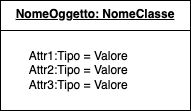
\includegraphics[scale=0.7]{img/diagrammaoggetti.png}
\end{wrapfigure}
In questo caso, un collegamento tra \emph{oggetti} è un'\textbf{\textcolor{cyan}{istanza d'associazione}}, non ha un nome
ma si possono indicare i ruoli. Inoltre non esiste la molteplicità, in quanto è sempre $1$ a $1$.